\documentclass[UTF8,a4paper,10pt]{ctexart}

\usepackage[margin=2.0cm]{geometry}
\usepackage{graphicx}
\usepackage{booktabs}
\usepackage{array}
\usepackage{tabularx}
\usepackage{longtable}
\usepackage{xcolor}
\usepackage{caption}
\usepackage{enumitem}
\usepackage{hyperref}
\hypersetup{colorlinks=true,linkcolor=blue!50!black,urlcolor=blue!50!black}
\captionsetup{font=small}
\setlist{nosep,leftmargin=1.6em}

\setCJKmainfont{Noto Serif CJK SC}
\setCJKsansfont{Noto Sans CJK SC}
\setCJKmonofont{Noto Sans Mono CJK SC}

\newcommand{\code}[1]{\texttt{\detokenize{#1}}}
\newcommand{\yes}{\textcolor{green!45!black}{是}}
\newcommand{\no}{\textcolor{red!65!black}{否}}

\title{\heiti 第三轮报告：在无循环的流程平台上\\用人工结构修复 AutomationBench 失败任务}
\author{霍建杰\\ \small 分支 \code{feature-wonder} · 2026-11-25}
\date{}

\begin{document}
\sloppy
\setlength{\emergencystretch}{3em}
\maketitle

\begin{abstract}
本轮目标是在 \code{rsi-flow-platform} 上人工编排结构，修复 AutomationBench 中至少 10 个具体问题，
并为下一阶段“LLM 生成结构”铺路。平台原生不支持循环：引擎的 \code{Executor} 是 DAG 队列，
画布没有循环容器。我们在结构层定义了 \code{loop} 节点（forEach/while/retry、预算、状态、嵌套、checkpoint），
在后端实现解释器执行它，并把画布 JSON 接到后端。最终 10 个失败任务全部从基线提升到
\code{partial_credit = 1.0}（56/56 断言），且 \textbf{没有调用任何模型}。
消融显示去掉循环后 QB 降到 0.4、Mailchimp 降到 0.286；2 道 held-out 迁移题零新增节点通过；
节点库 108 个实例仅 12 种类型，复用率 92\%。本报告同时给出失败边界、下一阶段 LLM 生成契约与复现方式。
\end{abstract}

\tableofcontents
\clearpage

\section{目标与结论}

\subsection{目标}
来自 \code{notes/target.md}：
\begin{enumerate}
  \item 从 AutomationBench 挑至少 10 个可判定问题，写清输入、期望、失败原因；
  \item 设计带循环的编排结构：重复条件、终止条件、状态存放，长序列不丢上下文；
  \item 在 \code{rsi-flow-platform} 上人工编排并跑通；
  \item 失败反馈：哪些没修好、为什么；
  \item 下一阶段：让 LLM 自主生成结构。
\end{enumerate}

\subsection{结论}
\begin{itemize}
  \item 10 个主任务全部 \code{1.0}，基线平均 0.426，断言 56/56；
  \item 10 题均通过平台“运行”按钮执行，每题有截图；
  \item 循环语义有实现、有测试（终止/预算/状态/checkpoint/嵌套）；
  \item 消融与迁移证明提升来自结构，不是模型；
  \item 局限与未做项在第~\ref{sec:limits} 节如实列出。
\end{itemize}

\section{现状：平台原生没有循环}

\begin{table}[h]
\centering
\small
\begin{tabularx}{\textwidth}{lXX}
\toprule
位置 & 现状 & 证据 \\
\midrule
\code{rsi-flow} 引擎 & \code{Executor} 是 \code{Queue<Source>}，按 routes 入队出队，无回边 &
\code{Executor.java} \\
节点校验 & 参数/结果只在流程开始、节点结束各校验一次 & \code{FlowHolder} \\
画布 & 只有元素与连线，没有循环容器/回边语义 & \code{rsi-flow-visual} \\
\bottomrule
\end{tabularx}
\end{table}

因此循环不能靠“画一条回去的线”实现，必须在结构层定义显式 \code{loop} 节点，由解释器执行。
本轮\textbf{没有修改} \code{rsi-flow} 引擎。

\section{循环语义设计}

\subsection{三种模式}
\begin{table}[h]
\centering
\small
\begin{tabularx}{\textwidth}{lXX}
\toprule
模式 & 重复条件 & 用途 \\
\midrule
\code{forEach} & \code{items} 还有下一个 & 逐行/逐条处理（10 题主要用法） \\
\code{while} & \code{condition} 为真 & 轮询、条件循环 \\
\code{retry} & 上次失败且未超次数 & 工具瞬时错误重试 \\
\bottomrule
\end{tabularx}
\end{table}

\subsection{帧与状态}
解释器维护循环帧：
\begin{verbatim}
frame = { index, count, current, state }
vars["loop"] = frame
vars[itemVar] = items[index]
vars[indexVar] = index
\end{verbatim}
状态分开存放：当前项/索引在变量表；累加器在 \code{frame.state}；
每轮日志在 \code{perIteration}；快照在 \code{checkpoints}（内存环形 + 可选 JSONL）；
最终汇总写入 \code{loop_<id>}，下游可用 \code{{{loop_loop1.state.summary}}} 读取。

\subsection{终止与预算}
\textbf{五个终止来源，先到先停：}
\begin{enumerate}
  \item 集合耗尽 / \code{condition} 为假 $\rightarrow$ \code{DONE}
  \item \code{breakWhen} $\rightarrow$ \code{BROKEN}
  \item \code{maxIterations}（默认 \code{max(50, N)}，硬上限 300）$\rightarrow$ \code{EXHAUSTED}
  \item \code{budget.wallClockMs} $\rightarrow$ \code{TIMEOUT}
  \item \code{budget.maxFailures} / \code{onError=abort} $\rightarrow$ \code{FAILED}
\end{enumerate}
\textbf{不允许静默截断}：\code{EXHAUSTED/TIMEOUT/FAILED} 默认让整体结构失败，
除非节点声明 \code{allowPartial: true}。

\subsection{嵌套与失败}
\begin{itemize}
  \item 嵌套最多 2 层，加载时校验（三层直接拒绝）；
  \item \code{onError: continue / abort / retry}；失败记录 \code{index/item/error}；
  \item \code{checkpoint: \{every, keep, file\}}：内存环形 + 磁盘 JSONL 全量。
\end{itemize}

\section{系统实现}

\subsection{架构}
\begin{verbatim}
浏览器 platform: getView -> {meta,nodes,edges}
   POST /flowTesting-core/api/engine/flow
后端 :39910 FlowCodeRun -> StructureExecutor
   fetch/action -> BridgeClient -> bridge /tool (Python WorldState)
   loop/branch/... 在 Java 执行
   结束 -> bridge /score -> result JSON
前端 -> 结果面板 status/score/assertions
\end{verbatim}

\subsection{后端代码}
\begin{longtable}{p{0.30\textwidth}p{0.10\textwidth}p{0.52\textwidth}}
\toprule
文件 & 行数 & 职责 \\
\midrule
\code{FlowCodeRun.java} & -- & 接收 structure，调用解释器，取分，写 result \\
\code{StructureExecutor.java} & 583 & 解析/校验/节点分发/数据与动作节点 \\
\code{LoopRunner.java} & 204 & 循环帧、终止、预算、状态、checkpoint \\
\code{NodeSupport.java} & 90 & 数组/数字/模板/item 绑定/JSONL \\
\code{Expr.java} & 72 & JEXL 求值 + \code{{{}}} 模板 \\
\code{BridgeClient.java} & 96 & \code{/tool} 与 \code{/score} \\
\code{FlowCodeFetch.java} & 45 & \code{FLOW_SKILL_FETCH} 的引擎执行 \\
\bottomrule
\end{longtable}

\subsection{节点}
实现了 16 种节点：
\code{fetch}、\code{rows}、\code{filter}、\code{map}、\code{aggregate}、
\code{loop}、\code{branch}、\code{action}、\code{encode}、\code{compute}、
\code{datediff}、\code{businessdays}、\code{join}、\code{collect}、
\code{first}、\code{assert}。
前端画布元素 \code{pendant.node} 存节点，\code{pendant.meta} 存任务信息；
链路边变成 \code{edges}，循环体/分支体用 \code{edge:false} 的虚线。

\subsection{平台闭环}
\code{structures.ts} 由 \code{structures/*.json} 生成，
\code{buildTest.tsx} 生成画布；点“运行”后 \code{getView} 收集
\code{nodes/edges/meta} 发给后端。10 题全部通过平台运行并得分，
结果见 \code{results/platform-runs.csv}。

\begin{figure}[h]
\centering
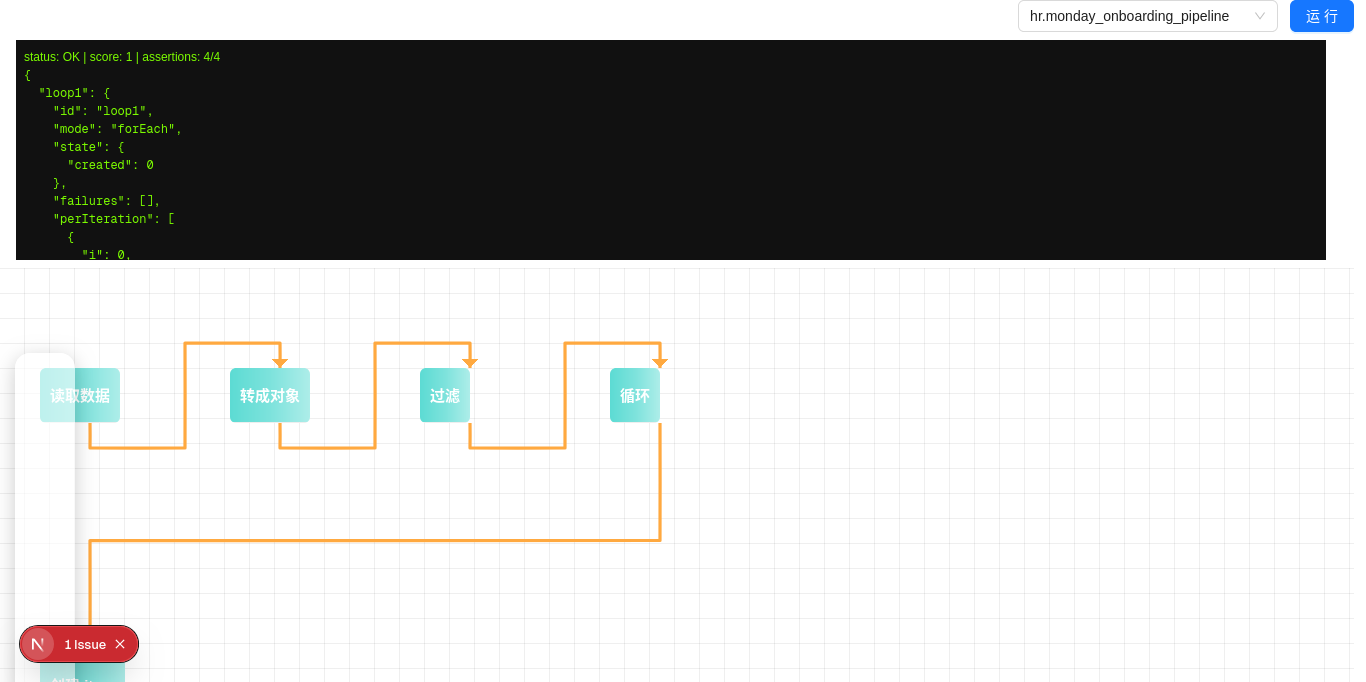
\includegraphics[width=0.92\textwidth]{../results/platform-score-monday.png}
\caption{平台运行 Monday 任务：结果面板显示 \code{status: OK | score: 1 | assertions: 4/4}。}
\end{figure}

\section{10 个任务的结果}

\begin{table}[h]
\centering
\small
\begin{tabular}{rlcccc}
\toprule
\# & 任务 & 基线 & 结构 & 断言 & 轮次 \\
\midrule
1 & \code{hr.monday_onboarding_pipeline} & 0.00 & 1.0 & 4/4 & 2 \\
2 & \code{finance.qb_invoice_from_orders} & 0.00 & 1.0 & 5/5 & 3 \\
3 & \code{finance.revenue_recognition} & 0.75 & 1.0 & 3/3 & 2 \\
4 & \code{hr.policy_update_distribution} & 0.25 & 1.0 & 4/4 & 2 \\
5 & \code{sales.overdue_followup_flag} & 0.44 & 1.0 & 9/9 & 7 \\
6 & \code{operations.space_utilization_analysis} & 0.60 & 1.0 & 5/5 & 3 \\
7 & \code{hr.zoom_orientation_sessions} & 0.67 & 1.0 & 6/6 & 3 \\
8 & \code{finance.vendor_insurance_verification} & 0.83 & 1.0 & 6/6 & 4 \\
9 & \code{operations.mailchimp_ecommerce_sync} & 0.71 & 1.0 & 7/7 & 7 \\
10 & \code{finance.payment_terms_tracking} & 0.00 & 1.0 & 7/7 & 5 \\
\midrule
 & 合计/平均 & 0.426 & 1.000 & 56/56 & 38 \\
\bottomrule
\end{tabular}
\end{table}

\subsection{为什么能修好}
\begin{itemize}
  \item \textbf{失败主要是“覆盖”而不是“理解”}：0 分的题都是“没做/只做第一条”；
  \item \textbf{过滤决定正确性}：排除 Cancelled、Inactive、refund/internal/opt-out、不应写出的行；
  \item \textbf{分支决定“做不做”}：5 题用条件路由；
  \item \textbf{规则来自人读证据}：Carol 搬回 Austin、2B-105 新团队入驻、
        Pinnacle Net 20、CloudHost Net 30 等。
\end{itemize}

\section{消融与迁移}

\subsection{消融：去掉循环}
\begin{table}[h]
\centering
\small
\begin{tabular}{lccc}
\toprule
任务 & 完整结构 & 只处理第一条 & 差值 \\
\midrule
\code{finance.qb_invoice_from_orders} & 1.0（5/5） & 0.4（2/5） & $-0.60$ \\
\code{operations.mailchimp_ecommerce_sync} & 1.0（7/7） & 0.286（2/7） & $-0.714$ \\
\bottomrule
\end{tabular}
\end{table}

\subsection{迁移：held-out 新题}
\begin{table}[h]
\centering
\small
\begin{tabular}{lcccc}
\toprule
迁移题 & 基线 & 迁移后 & 断言 & 新增节点类型 \\
\midrule
\code{support.zoho_multitenant_isolation} & 0.75 & 1.0 & 16/16 & 0 \\
\code{marketing.analyst_mention_tracking} & 0.917 & 1.0 & 12/12 & 0 \\
\bottomrule
\end{tabular}
\end{table}

\subsection{节点复用}
10 个主任务共 108 个节点实例、12 种类型，复用率 92\%：

\begin{table}[h]
\centering
\small
\begin{tabular}{lcc}
\toprule
节点类型 & 任务数 & 说明 \\
\midrule
\code{action/fetch/loop} & 10 & 全部任务 \\
\code{rows} & 9 & 除 overdue \\
\code{encode/filter} & 8 & 多数任务 \\
\code{branch} & 5 & 条件路由 \\
\code{collect} & 4 & 汇总到 state \\
\code{compute/datediff/join} & 2 & 计算/日期/关联 \\
\code{businessdays} & 1 & 控制原语，参数无法表达 \\
\bottomrule
\end{tabular}
\end{table}

\section{长序列与循环测试}

\begin{table}[h]
\centering
\small
\begin{tabularx}{\textwidth}{lX}
\toprule
用例 & 结果 \\
\midrule
120 项 forEach & 120 轮，120 条 \code{perIteration} \\
checkpoint（every=5, keep=20） & 内存 20 条；磁盘 JSONL 24 条（含淘汰） \\
\code{allowPartial} & 超限默认 \code{ERROR}；声明后 \code{OK + partial} \\
\code{maxFailures=2} & 循环 \code{FAILED}，整体 \code{ERROR} \\
\code{wallClockMs=1} & \code{TIMEOUT}，10 轮后停 \\
\code{while i<3} & 3 轮 \code{DONE} \\
\code{retry} & 1 成功 2 失败，每项重试 2 次 \\
三层嵌套 & 加载时拒绝 \\
\bottomrule
\end{tabularx}
\end{table}

\section{失败反馈与限制}
\label{sec:limits}

\begin{itemize}
  \item 最终 10/10 没有失败项；备用 \code{finance.invoice_email_extract}（缺 LLM 抽取节点）
        和 \code{support.zendesk_sf_case_sync}（三表配置 + diff，时间不够）没有做；
  \item \textbf{反例}：payment terms 只信表格（不读邮件/Slack）得 0.571，
        说明人工读证据不可替代；
  \item \textbf{断言通过 $\neq$ 语义完整}：QB 的 10\% 折扣、QuickBooks 实际更新、
        Notion 正文、部分 Slack 文案没有完全实现，只是断言不查；
  \item 负向断言被官方默认排除；我们尽量满足，但评分不检查；
  \item 迁移样本只有 2 道；基线/结构都是单次运行，没有方差；
  \item 循环设计里的 skill flow 只实现了 fetch，其余 action 直连 bridge；
  \item 平台只能演示，节点参数不能在线编辑。
\end{itemize}

\section{下一阶段：LLM 生成结构}

\subsection{输入}
任务 prompt、表头 + 样例行、工具目录、结构 schema、模式库、2--3 个示例、硬约束。

\subsection{约束}
节点白名单；嵌套 $\le 2$；每个 loop 必须有终止；写操作前必须过滤；
LLM 不控制循环；schema 校验通过才执行；不可逆动作需人工确认。

\subsection{判定}
语法/schema $\rightarrow$ 执行 \code{status=OK} $\rightarrow$ 官方 \code{partial_credit}
$\rightarrow$ 人工抽查“每个节点能对应任务要求”。

\subsection{哪些必须人工}
业务规则解释（邮件/Slack 证据）、验收标准、API 端点确认、不可逆动作、失败归因。
下一阶段目标不是“全自动”，而是量化“LLM 能替代多少人工”。

\section{AI 使用与核实}

\textbf{AI 做了什么}：读数据、定位断言、起草结构 JSON、实现解释器、跑 harness、写文档。\\
\textbf{人做了什么}：决定每题结构与规则、确认断言与语义、能逐题解释为什么这样编排。\\
\textbf{怎么核实}：官方 \code{partial_credit}、平台 10/10 截图、消融/迁移、循环语义测试。\\
\textbf{边界}：不是 LLM 端到端生成结构；10 题没有调用模型。

\section{复现}

\begin{verbatim}
# 结构导出到平台
python3 loop-structures/harness/export_platform_structures.py

# 单题跑分（自动起停 bridge）
cd loop-structures
python3 harness/run_structure.py \
  --structure structures/hr.monday_onboarding_pipeline.json --restart-bridge

# 10 题全部从平台 UI 跑（需 backend :39910 + dev :3000 + geckodriver）
python3 harness/platform_run.py

# 汇总
python3 harness/summarize_results.py
python3 harness/node_usage.py
\end{verbatim}

后端启动参数、bridge 启动方式、MySQL 配置见仓库 \code{docs/00-presentation-guide.md} 与
\code{notes/env-repro.md}。凭据不写入仓库。

\appendix
\section{文件索引}
\begingroup\footnotesize
\begin{longtable}{p{0.44\textwidth}p{0.50\textwidth}}
\toprule
路径 & 内容 \\
\midrule
\path{loop-structures/docs/01-loop-design.md} & 循环语义 \\
\path{loop-structures/docs/02-node-taxonomy.md} & 节点分层/准入 \\
\path{loop-structures/docs/03-patterns.md} & P1--P6 模式 \\
\path{loop-structures/docs/04-design-rationale.md} & 10 题编排理由 \\
\path{loop-structures/docs/05-reuse.md} & 消融/迁移/节点统计 \\
\path{loop-structures/docs/06-llm-generation.md} & LLM 生成契约 \\
\path{loop-structures/docs/07-platform.md} & 平台闭环 \\
\path{loop-structures/docs/08-long-sequence.md} & 长序列 \\
\path{loop-structures/docs/09-results.md} & 10 题结果 \\
\path{loop-structures/docs/10-limitations.md} & 失败反馈 \\
\path{loop-structures/docs/11-loop-tests.md} & 循环测试 \\
\path{loop-structures/docs/12-code-walkthrough.md} & 逐行代码走读 \\
\path{loop-structures/structures/} & 10 题 + 消融/迁移/压力 \\
\path{loop-structures/results/} & CSV、每题 JSON、平台截图 \\
\path{loop-structures/harness/} & 运行器/统计/导出 \\
\path{loop-structures/schema/structure.schema.json} & 结构 schema \\
\bottomrule
\end{longtable}
\endgroup

\end{document}
